\documentclass[11pt, twoside, a4paper, titlepage]{article}

% credits
% - https://www.youtube.com/watch?v=-TRcPIPkZz8

% for formatting
\usepackage[most]{tcolorbox}

% for icons
\usepackage[width=0.3cm]{svg}

% for links
\usepackage[colorlinks=true, allcolors=blue]{hyperref}

%for media
\usepackage{graphicx}
\graphicspath{ {./Media/} }

% for setting margins
\usepackage{geometry}
\geometry{
	a4paper,
	left=0.1cm,
	right=0.1cm,
	top=0.1cm,
	bottom=0.1cm
}

\author{Miro Noordzij}
\title{Miro Noordzij | Software Engineer}

\begin{document}

\tcbset{colframe=black, colback=white, arc=0mm, sharp corners}
\begin{tcolorbox}[boxsep=0mm, left=0mm, right=0mm, top=0mm, bottom=0mm]
	\begin{minipage}{6cm}
		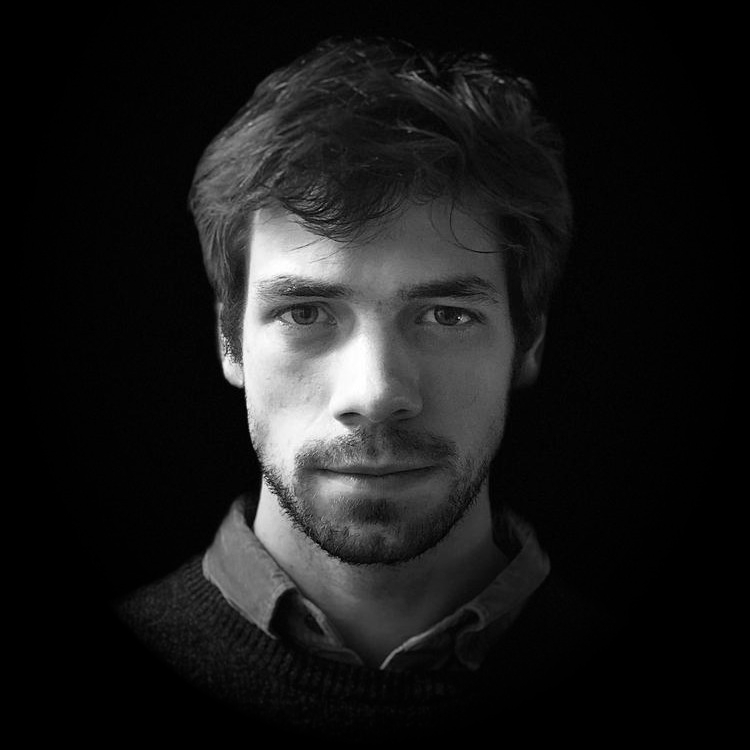
\includegraphics[width=6cm, height=6cm ]{avatar.jpg}
	\end{minipage}
	\begin{minipage}{14.8cm}
		\begin{center}
			\Huge
			\textbf{Miro Noordzij}  Software Developer
			\vspace*{0.3cm}\\
			\small
			\parbox{14cm}{Software Developer based in Rotterdam with experience in embedded systems and web development. Passionate about technology and committed to continuous learning, always exploring new frameworks, programming languages, and development methodologies such as the mantras of clean code. Outside of work, I enjoy sailing, making music, and staying active at the gym.}
			\vspace*{0.3cm}\\
			\includesvg{LinkedIn.svg}
			\href{https://www.linkedin.com/in/miroaccli}{miroaccli} |
			\includesvg{GitHub.svg}
			\href{https://www.github.com/miroaccgh}{miroaccgh} |
			\includesvg{Website.svg}
			\href{https://www.kaizen.red}{kaizen.red} \\
			\includesvg{Email.svg}
			\href{mailto:mironoordzij@outlook.com}{mironoordzij@outlook.com} |
			\includesvg{Phone.svg}
			\href{tel:+31653904797}{+31 6 53904797} |
			\includesvg{Home.svg}
			\href{https://g.co/kgs/Ak21VtP}{Rotterdam, The Netherlands}
		\end{center}
	\end{minipage}
\end{tcolorbox}

\vspace{-0.6cm}

\begin{tcolorbox}[boxsep=0mm, left=0mm, right=0mm, top=0mm, bottom=0mm, height=23cm]
	\begin{minipage}[t]{6.01cm}
		\begin{tcolorbox}[colframe=black, colback=black, arc=0mm, sharp corners, fontupper=\color{white}, height=22.9cm]
			\section*{Skills}
			
			\subsection*{Technical}
			\textbf{Languages}\\
			\large{Sufficient}\\
			\small
			\parbox{5cm}{Python • Shell/BASH • SQL \\ HTML • CSS }
			
			\vspace*{0.2cm}
			
			\large{Familiar}\\
			\small
			\parbox{5cm}{C++ • Typescript/Javascript \\ Latex • Nix • PHP }
			
			\vspace*{0.4cm}
			
			\textbf{Frameworks}\\
			\parbox{5cm}{Flask • React}
			
			\vspace*{0.4cm}
			
			\textbf{Tools \& Platforms}\\
			\parbox{5cm}{Git/CLI • AWS • Linux/NixOS  MongoDB • MySQL • Azure \\ Docker • Node.js • Docker \\ Arduino • Atlasian • MQTT \\ Redis • Blender • Poetry }
			
			\vspace*{0.4cm}
			
			\textbf{Methodology \& Principles}\\
			\parbox{5cm}{SOLID • SCRUM • 5S • TDD }
			
			\subsection*{General}
			
			\textbf{Languages}\\
			\begin{itemize}
				\item Dutch: Native
				\item English : Bilingual
			\end{itemize}
			
			\vspace*{0.4cm}

			\textbf{Certificates}\\
			\begin{itemize}
				\item EHBO
				\item BHV
			\end{itemize}
			
			\vspace*{0.4cm}


			\textbf{References}\\
			\begin{itemize}
				\item{ Nilesh Debi\\
					Software Developer\\
					@\href{https://www.truefullstaq.com/}{TrueFullStaq}\\
					Tel: \href{tel:+31637016271}{+31 6 37016271}\\
					LinkedIn: \href{https://www.linkedin.com/in/nilesh-kd}{nilish-kd}}
				\item{ Robert Saunders\\
					Senior Software Developer\\
					@\href{https://www.eyeconcept.nl/}{Eye Concept}\\
					Tel: \href{tel:+31653742508}{+31 6 53742508}\\
					LinkedIn: \href{https://www.linkedin.com/in/robert-ronald-saunders}{robert-ronald-saunders}}
			\end{itemize}
		\end{tcolorbox}
	\end{minipage}
	\vspace*{-0.3cm}
	\begin{minipage}[t]{14cm}
		\begin{tcolorbox}[grow to left by=0.0cm, colframe=white, colback=white, height=22.9cm]
			\section*{Education}
			\textbf{University of Applied Sciences Rotterdam}\\
			\emph{HBO AD Software Development, 2021-2025}
			
			\vspace*{0.3cm}
			
			\textbf{Grafisch Lysceum Rotterdam}\\
			\emph{MBO AV-Specialist, 2017-2021}
			
			\vspace*{0.3cm}
			
			\textbf{Het Lyceum Rotterdam}\\
			\emph{HAVO, 2012-2017}
			
			\section*{Experience}
			\textbf{Trainee Software Developer}\\
			\emph{Eye-Concepts, 2025-NOW}\\
			\parbox{13cm}{Currently I'm developing microservices for a real time operating system for cranes. In this I gain a lot of experience and knowledge in the field of platform engineering and cloud computing For this I use Azure DevOps Tools, MQTT and Python.}
			\parbox{13cm}{ MQTT • TDD • Python • Azure • DevOps • Microservices SOLID • Redis }
			
			\vspace*{0.3cm}
			
			\textbf{IoT Technical Support Officer}\\
			\emph{Fortes ES12, 2024-2024}\\
			\parbox{13cm}{I provided technical support and consult over thousends of IoT, setup a knowledge base and ticketing system, analyzed incoming data and learned a lot about various protocols and tools.}
			\parbox{13cm}{ Atlassian • Python • IoT • Excel }
			
			\vspace*{0.3cm}
			
			\textbf{Embedded Software Developer}\\
			\emph{Finder Relays, 2023-2024}\\
			\parbox{13cm}{At this internship I designed an energy management and monitoring system. It tracked the harnessed energy from solarpanels. In case of an overcapacity it would make a passive heating system active. I configured the electronics, logic, piping and developed the dashboard.}
			\parbox{13cm}{ C++ • Python • Arduino • Sensors • Electronics • Pipes • ADC }
			
			\vspace*{0.3cm}
			
			\textbf{Software Developer}\\
			\emph{Dyflexis, 2022-2023}\\
			\parbox{13cm}{My first professional position as a developer. Although I worked within a scrum team with an agile methodolgy during studies, I would say this position was my true introduction to working actively within a scrum team with an elaborate SDLC and CI/CD Pipeline.}
			\parbox{13cm}{ PHP • Symfony • JavaScript • Vue.js • SQL • Docker • GitLab }
			
			\vspace*{0.3cm}
			
			\textbf{Trainee Software Developer}\\
			\emph{Mytronics, 2021-2021}\\
			\parbox{13cm}{At this agri-tech start-up my role was to create show-cases and demos for a prototype smart camera, in return for my work I got lessons in software development from the CEO, CTO, CFO etc.}
			\parbox{13cm}{ Python • Blender }
		\end{tcolorbox}
	\end{minipage}
\end{tcolorbox}

\vspace*{-0.1cm}

\small
\emph{ I developed this resume using \href{https://www.latex-project.org/}{Latex} to demonstrate my skills, all blue text are links and you can check its repo out on my GitHub. }
\end{document}